\documentclass{book}
\usepackage[inner=1.2in, outer=1in, top=1.2in, bottom=1.2in]{geometry}
\author{akshat}
\date{2020}

\setcounter{tocdepth}{3}
\setcounter{secnumdepth}{3}

%%% Landscape
\usepackage{pdflscape}

%%% Content in multiple columns
\usepackage{multicol}

%%% Colors
\usepackage[dvipsnames]{xcolor}

%%% Text Spacing
\usepackage{setspace}

%%% Maths
\usepackage{amsmath}

%%% Packages for tables
\usepackage{arydshln}
\usepackage{multirow}
\renewcommand{\arraystretch}{1.5}

%Packages for Figures
\usepackage{graphicx}
\setlength{\fboxrule}{2pt}

%Packages for Subfigures
\usepackage{caption}
\usepackage{subcaption}

\usepackage{float}

\begin{document}
	

    \chapter{Introduction}
    \pagenumbering{arabic}
    \setcounter{page}{1}
    
    \begin{doublespace}
    With the advance of big data analytics equipment, more devotion has been paid to disease expectation from the perception of big data inquiry, various experiment have been conducted by choosing the features mechanically from a large number of data to improve the truth of menace classification rather than the formerly selected physiognomies. However, those prevailing work mostly measured structured data. Number of researches have been conducted to select the characteristics of a disease prediction from a large volume of data. Most of the existing work is based on  structured data. For the unstructured data one can use a convolutional neural network. Convolutional neural networks are made up of a neuron, each neuron receives some inputs and performs operations and the whole network expresses a single differentiable score function.
    
    The system analyses the structured and unstructured data in the healthcare field to assess the risk of disease. First, it uses Decision tree map algorithm to generate the pattern and causes of disease. Second, by using Map Reduce algorithm for partitioning the data such that a query will be analyzed only in a specific partition, which will increase the operational efficiency but reduce query retrieval time. Map reducing algorithm is used for partitioning the medical data based on the output of Decision Tree map algorithm. Compared to several typical prediction algorithms, the prediction accuracy of our proposed algorithm increases.
    
    The primary aim of this project is to analyze the “Pima Indian Diabetes Dataset” and “Cleveland Heart Disease Dataset” and use Logistic Regression, Support Vector Machine, Naïve Bayes, K-Nearest Neighbors and Multi-Layer Perceptron (Neural Network) for prediction and develop a prediction engine. Using structured and unstructured data from hospital it uses Machine Learning Decision Tree algorithm and Map Reduce algorithm. To the best of our knowledge in the area of medical big data analytics none of the existing work focused on both data types.
    \end{doublespace}
    	
    \section{Background Study}
    \subsection{Motivation}

    \paragraph{}
    The main motivation of doing this research is to present a heart disease prediction model for the prediction of occurrence of heart disease. Further, this research work is aimed towards identifying the best classification algorithm for identifying the possibility of heart disease in a patient. This work is justified by performing a comparative study and analysis using three classification algorithms namely Naïve Bayes, Decision Tree, KNN, Logistic Regression and Random Forest are used at different levels of evaluations. Although these are commonly used machine learning algorithms, the heart disease prediction is a vital task involving highest possible accuracy. Hence, the three algorithms are evaluated at numerous levels and types of evaluation strategies. This will provide researchers and medical practitioners to establish a better understanding and help them identify a solution to identify the best method for predicting the heart diseases.
    \paragraph{}
    A key challenge confronting healthcare organization (hospitals, medical centers) is the facility of quality services at reasonable prices. Quality amenities suggest diagnosing patients accurately and regulating medications that are effective. Poor clinical choices can prompt deplorable results, which are in this manner unsatisfactory. Hospitals should limit the cost of clinical tests. They can accomplish these outcomes by utilizing fitting PC based data and additionally choice emotionally supportive networks. The heart is the essential piece of our body. Life is itself reliant on effective working of the heart. If task of the heart isn't legitimate, it will influence the other body parts of human, for example, cerebrum, kidney and so on. Coronary illness is a sickness that effects on the activity of the heart.
     \paragraph{}
    There are several elements which builds danger of Heart ailment. Some of them are listed below:
    \begin{itemize}
    	\item The family history of heart disease
    	\item The family history of heart disease
    	\item The family history of heart disease
    	\item Smoking
    	\item Cholesterol
    	\item High blood pressure
    	\item Obesity
    	\item Lack of physical exercise
    \end{itemize}
    \paragraph{}
    Because of a wide accessibility of superlative measure of information and a need to change over this accessible huge measure of information to helpful data requires the utilization of information mining strategies. Information Mining and KDD (learning disclosure in the database) have turned out to be prominent as of late. The popularity of information mining and KDD (information revelation in database) shouldn't be an amazement since the measure of the information increases that are accessible are extremely extensive to be analyzed physically and even the techniques for programmed information investigation in view of established insights and machine adapting frequently threaten issues when preparing large, dynamic information increases comprising of complex items [12]. Information Mining is the center piece of Knowledge Discovery Database (KDD). Numerous individuals regard Data Mining as an equivalent word for KDD since it's a key piece of KDD process. There are sure stages of information mining that you will need to get comfortable with, and these are exploration, pattern identification, and deployment. Information mining is an iterative procedure that commonly includes the accompanying stage.
    \pagebreak
    \begin{itemize}
    	\item About 23 lakh people die of heart disease in India every year, that’s 1 in every 4 deaths.
    	\item Heart disease is the leading cause of death for both men and women. More than half of the deaths due to heart disease in the year 2009 were in men.
    	\item In the India, someone has a heart attack every 40 seconds.
    	\item 1\% of women of age 40 who participate in routine screening have heart problems.
    	\item A lot of amount is spent by the government on the patients diagnosed with heart diseases. The amount spent includes the cost of healthcare services, medications, and lost productivity.
    \end{itemize}
    
    \subsection{Social Impact}
    In day to day life many factors that affect a human heart. Many problems are occurring at a rapid pace and new heart diseases are rapidly being identified. In today’s world of stress Heart, being an essential organ in a human body which pumps blood through the body for the blood circulation is essential and its health is to be conserved for a healthy living. The health of a human heart is based on the experiences in a person’s life and is completely dependent on professional and personal behaviors of a person. There may also be several genetic factors through which a type of heart disease is passed down from generations. According to the World Health Organization, every year more than 12 million deaths are occurring worldwide due to the various types of heart diseases which is also known by the term cardiovascular disease. The term Heart disease includes many diseases that are diverse and specifically affect the heart and the arteries of a human being. Even young aged people around their 20-30 years of lifespan are getting affected by heart diseases. The increase in the possibility of heart disease among young people may be due to the bad eating habits, lack of sleep, restless nature, depression and numerous other factors such as obesity, poor diet, family history, high blood pressure, high  blood cholesterol, idle behavior, family history, smoking and hypertension.  The diagnosis of heart diseases is very important and is itself the most  complicated task in the medical field. All the mentioned factors are taken into consideration when analyzing and understanding the patients by the doctor through manual check-ups at regular intervals of time.
    \paragraph{}
    The symptoms of heart disease greatly depend upon which of the discomfort felt by an individual. Some symptoms are not usually identified by the common people. However, common symptoms include chest pain, breathlessness, and heart palpitations. The chest pain common to many types of heart disease is known as angina, or angina pectoris, and occurs when a part of the heart does not receive enough oxygen. Angina may be triggered by stressful events or physical exertion and normally lasts under 10 minutes. Heart attacks can also occur as a result of different types of heart disease. The signs of a heart attack are like angina except that they can occur during rest and tend to be more severe. The symptoms of a heart attack can sometimes resemble indigestion. Heartburn and a stomach ache can occur, as well as a heavy feeling in the chest. Other symptoms of a heart attack include pain that travels through the body, for example from the chest to the arms, neck, back, abdomen, or jaw, lightheadedness and dizzy sensations, profuse sweating, nausea and vomiting.
    \paragraph{}
    Heart failure is also an outcome of heart disease, and breathlessness can occur when the heart becomes too weak to circulate blood. Some heart conditions occur with no symptoms at all, especially in older adults and individuals with diabetes. The term 'congenital heart disease' covers a range of conditions, but the general symptoms include sweating, high levels of fatigue, fast heartbeat and breathing, reathlessness, chest pain. However, these symptoms might not develop until a person is older than 13 years. In these types of cases, the diagnosis becomes an intricate task requiring great experience and high skill. A risk of a heart attack or the possibility of the heart disease if identified early, can help the patients take  precautions and take regulatory measures. Recently, the healthcare industry has been generating huge amounts of data about patients and their disease diagnosis reports are being especially taken for the prediction of heart attacks worldwide. When the data about heart disease is huge, the machine learning techniques can be implemented for the analysis.
    
    
    \section{Related Work}
    The healthcare industry collects huge amounts of healthcare data which, unfortunately, are not ``mined" to discover the hidden information for effective decision making. Discovery of hidden patterns and relationships often goes unexploited.
    The healthcare environment is still ‘information rich’ But ‘knowledge poor’. There is a wealth of data available within the health care systems. However, there is a lack of effective analysis tools to discover hidden relationships in data.
    Today medical services have come a long way to treat patients with various diseases. Among the most lethal one is the heart disease problem which cannot be seen with a naked eye and comes instantly when its limitations are reached. Today diagnosing patients correctly and administering effective treatments have become quite a challenge. This section provides the basic concepts of classifier as Naive Bayes and feature subset selection method as PSO.
   
    \subsection{Particle swarm optimization (PSO)}			
    PSO is an Evolutionary Computation technique proposed by Kennedy et al. in 1995. PSO is motivated by social behaviors such as bird flocking and fish schooling. In PSO population swarm consists of “n” particles, and the position of each particle stands for the potential solution in D-dimensional space. The particles change its condition based on three aspects: To keep its inertia; To change the condition according to its most optimist position; To change the condition according to the swarm’s most optimist position. In PSO, a population are encoded as particles in the search space dimensionality D.PSO starts with the random initialization of a population of particles. Based on the best experience of one particle (pbest) and its neighboring particles (gbest), PSO searches for the optimal solution by updating the velocity and the position of each particle; PSO is used as feature subset selection method due to its advantages:
    \begin{itemize}
    	\item Simple and easy to implement.
    	\item Continuous optimization approach.
    \end{itemize}
    
    \subsection{Naive Bayes Classifier}
    Naive Bayes classifiers are a family of simple probabilistic classifiers based by using Bayes theorem with strong (Naive) independence assumptions between the features. Naive Bayes classifiers are highly scalable by requiring several parameters linear for the number of features or predictors as variable in a learning problem.It is the simplest and the fastest probabilistic classifier especially for the training phase.	
    \linebreak
    \linebreak				
    \textbf{Feature selection} - It is a process of removing the irrelevant and redundant features from dataset based on evaluation criterion which is used to improve accuracy. There are two approaches as individual evaluation and other one is subset evaluation. The process of feature selection is classified into three broad classes. One is filter and another one is wrapper and third one is embedded method based on how the feature selection is deployed by supervised learning algorithm. In this paper, they proposed a model which uses Naive Bayes as classifier and PSO as Feature subset selection measure for prediction of heart disease.
    \linebreak
    \linebreak				
    \textbf{Proposed system} - In this section, we propose a methodology to improve the performance of Bayesian classifier for prediction of heart disease. Algorithm for our proposed model is shown below:
    \linebreak
    \linebreak
    \textbf{Algorithm 1: Heart disease prediction by using Bayes classifier and PSO.}
   	
    Input: Heart disease dataset.
    
    Output: Classify patient dataset into heart disease or not (normal).
    		
    Step 1: Read the dataset.
    
    Step 2: Apply particle swarm optimization for feature selection. 
    
    Step 3: Remove the features with low value of PSO.
    
    Step 4: Apply Naive Bayes classifier on relevant features. 
    
    Step 5: Evaluate the performance of NB+PSO model.
    
    \paragraph{}
    The above algorithm divided into two sections, section 1 (step 2 and step 3) performs processing and feature subset selection. In section 2 (step 4 and step 5) Naive Bayes is applied on relevant features data and evaluate the performance in terms of accuracy. Cross validation technique used to split into training and testing data.	    
    \begin{center}
    	Accuracy= (No. of objects correctly classified/Total no. of objects in test set)  	
    \end{center}
    
    
    \subsection{Datasets}
    For this project we have used The Cleveland heart dataset from the UCI Machine Learning Repository as it is widely used by the Pattern design community. The dataset consists of 303 individual clinical reports in which 164 did not have any disease. In this dataset there is a total of 97 female patients in which 25 people are the affirmative case, also there are 206 male patients in which 114 are diagnosed with the disease. There are 6 missing values in this dataset and all numeric values are recognized as numeric.
    We have 13 features that are relevant to the specific disease regarding the dataset shown below:
    \begin{itemize}
    	\item Age
    	\item Sex
    	\item Chest Pain Type
    	\item Resting Blood Pressure 
    	\item Serum Cholesterol in mg/dl 
    	\item Fasting Blood Sugar
    	\item Resting electrocardiographic result
    	\item Maximum heart rate achieved 
    	\item Exercised-induced angina
    	\item Old peak, ST depression induced by exercise relative to rest 
    	\item Number of major vessels colored by fluoroscopy 
    	\item Thal:3= Normal, 6=fixed defect, 7= reversible defect
    \end{itemize}
    The involvement of each attribute with respect to number of instances is as shown in the histogram below:
    
    \begin{figure}
	    	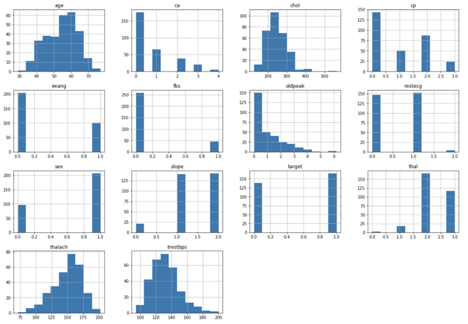
\includegraphics[]{images/histogram.png}
    \end{figure}
    
    
    \pagebreak
    The Count of each target class for the given dataset is as depicted below. The two target classes are:
    \begin{itemize}
    	\item 0: The instances that don’t have involvement in the disease prediction.
    	\item 1: The instances that have involvement in disease prediction.
    \end{itemize}

	\begin{figure}
			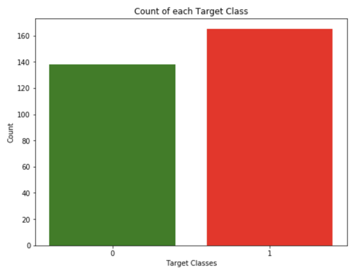
\includegraphics[]{images/count.png}
	\end{figure}

    
    
    
    \section{Summary of Gaps identified}
    Medical diagnosis is considered as a significant yet intricate task that needs to be carried out precisely and efficiently. The automation of the same would be highly beneficial. Clinical decisions are often made based on doctor’s intuition and experience rather than on the knowledge rich data hidden in the database. This practice leads to unwanted biases, errors and excessive medical costs which affects the quality of service provided to patients. Data mining has the potential to generate a knowledge-rich environment which can help to significantly improve the quality of clinical decisions.
    
       
    
    \section{Project problem statement and Objective}
    
    \subsection{Problem Statement}
    Doctors rely on common knowledge for treatment. When common knowledge is lacking, studies are summarized after some number of cases have been studied. But this process takes time, whereas if machine learning is used, the patterns can be identified earlier
    For using machine learning, a huge amount of data is required. There is a very limited amount of data available depending on the disease. Also, the number of samples having no diseases is very high compared to the number of samples actually having the disease.
    
    \subsection{Objectives of the project}
    1. The proposed system predicts heart diseases as well as the chances of diabetes.
    2. There are no proper methods to handle semi structured and unstructured data. The proposed system is expected to work well with both structured and unstructured data.
    3. The secondary objective of the project is to develop a web application which allows users to predict diabetes and heart disease using the prediction engine.
    
    
    \section{Organization of the Report}
    The rest of the report is organized as follows, Chapter 2 shows some high level designs, software development methodology and architecture, Chapter 3 tells about detailed design, data structures and algorithms used and UML diagrams, chapter 4 tells about the implementation level information,chapter 5 is about the testing the project functionality and chapter 6 is all about conclusion and future scope of the project.
    
    \chapter{High-level Design}
    
    This chapter covers the software engineering models on which this project is developed. Firstly, we describe briefly about the incremental model which included many cycles after which the current version of the Web App is achieved. Then, there is a description about agility which means regular check of the project status by the faculty panel and our respected guide. Then we describe briefly about scrum i.e., the regular meetings which the team members had.
    \section{Software Development Methodology}
    	Software Development Life Cycle (SDLC) is a technique used by the merchandise to configuration, make and trial top notch programming's (as appeared in figure 2.1). The SDLC means to send superb programming that meets or exceeds client desires, completes consummation inside conditions and cost instruments. SDLC is a technique took after for a product scheme, inside a product association. It includes of a nitty gritty preparation depicting how to create, keep up, displace and improve particular programming. The following diagram is a graphical illustration of the various stages of a typical SDLC.
    	
    	\begin{figure}
    		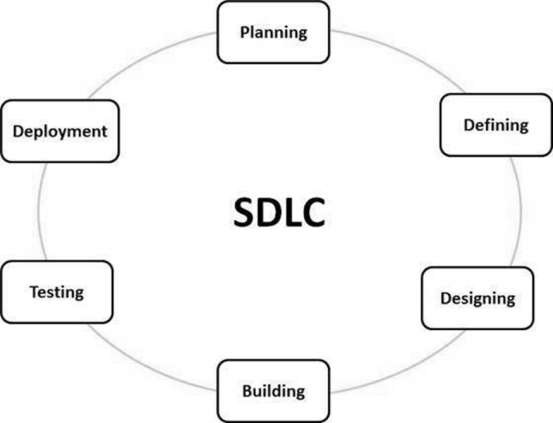
\includegraphics[]{images/sdlc.png}
    		
    		\begin{center}
    			Figure 2.1 Software Development Life Cycle
    		\end{center}
    	\end{figure}
    
    	\paragraph{}
    	The detailed SDLC diagram in this report show how all the stages has been collaborated to make the working of proposed work accurate and precise. 
    	A typical Software Development Life Cycle consists of the following stages:
    	
    	 \subsection{Stage 1: Planning and Requirement Analysis}
    	Requirement examination is one of the most essential and central stages in SDLC. It is done by the senior persons from the group with significant contributions from the client, the business office, advertise studies, space specialists in the business. This data is then made used for designing the essential undertaking approach and to direct item plausibility think about the effective, operational and specialized zones. Making courses of action for the quality affirmation necessities and recognizing evidence of the threats related with the wander is similarly done in the masterminding stage. The outcome of the particular good judgment considers is to depict the differing specific methods of insight that can be taken after to understand the errand adequately with minute perils.
    	
    	\subsection{Stage 2: Defining Requirements}
    	Once the essential examination is done the ensuing stage is to clearly portray and report the thing necessities and get them supported from the customer or the market agents. This is done through an SRS (Software Requirement Specification) report which contains all the thing essentials to be made and made in the midst of the undertaking life cycle.
    	
    	\subsection{Stage 3: Designing the Product Architecture}
    	An arrangement approach clearly describes all the plan modules of the thing close by its correspondence and data stream depiction with the external and untouchable modules (expecting any). Within framework of the significant number of modules of the proposed designing should be obviously described with the minutest of the inconspicuous components in DDS.
    	
    	\subsection{Stage 4: Building or Developing the Product}
    	In this period of SDLC the genuine change starts and the thing is made. The programming code is created by DDS in the midst of this stage. If the arrangement is performed in a positive and dealt with way, code age can be master absent much issue. Planners should take after the coding rules represented by their affiliation and programming gadgets like code compilers, middle people, checker debuggers, etcetera are made used to make the code. Differing anomalous state programming vernaculars, for instance, C, C++, Pascal, Java and Python are used for coding. The programming tongue is picked with respect to the sort of writing computer programs actually being delivered.
    	
    	\subsection{Stage 5: Testing the Product}
    	This stage is normally a subset of the extensive number of stages as in the front line SDLC models, the testing practices are generally connected with each one of the periods of SDLC. Regardless, this stage suggests the testing simply period of the thing represented, took after, settled and retested, until the point that the thing accomplishes the quality measures portrayed in the SRS.

    	\subsection{Stage 6: Deployment in the Market and Maintenance}
    	Once the thing is attempted and arranged to be passed on it is released formally in the correct market. Now and again thing sending happens in stages as indicated by the business strategy of that affiliation. The thing may first be released in a confined part and attempted in the certifiable business condition (UAT-User affirmation testing). By then in perspective of the info, the thing may be released as it is or with suggested changes in the concentrating on promote parcel. After the thing is released in the market, its upkeep is enhanced the circumstance the present customer base.
    	
    	\section{Architecture}
    	
    	\begin{figure}
    		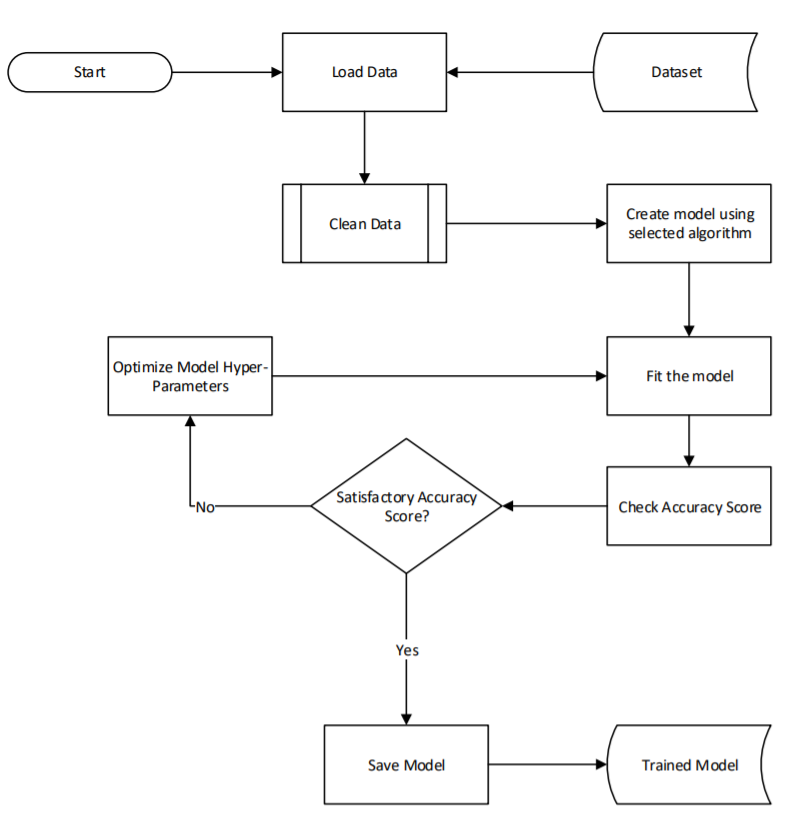
\includegraphics[]{images/df.png}
    		
    		\begin{center}
				Figure 2.2: Initial design of the proposed system
    		\end{center}
    	\end{figure}
    	
    	
    	This paper will provide as a result that is distributed into three phases:
    	
    	\begin{enumerate}
    		\item \textbf{Analysis Phase (Based on the Dataset): } In this stage the fundamental concentration is to the information from the dataset and do the examination in light of the medical data of the patient. In this stage we try to analyse which of the medical data or the medical values have more impact on the prediction of the disease and which attributes have the least impact.
    	\item \textbf{Combining analysis stage with the parameters:} In this stage we give a few parameters based on the condition of patient (whether the patient is suffering from heart disease and diabetes or not). The application then applies different machine learning algorithms to prepare a model which in turn is used in the prediction phase.  
    	\item \textbf{Prediction Phase::} In this stage we display the outcome and declare the probability that the person is suffering from heart disease or diabetes. The result predicted using different machine learning algorithms from the values given by the user.
    \end{enumerate}
    	
    	\section{Incremental Model}
    	
    	The incremental frame illustrate could be a strategy for programming movement where the thing is made, executed and endeavoured incrementally (to a few degrees more is consolidated each time) until the point that the thing is done (as showed up in figure 2.2). It joins both alter and back. The thing is depicted as wrapped up when it fulfills the more prominent portion of its necessities. This demonstrate consolidates the sections of the waterfall appear with the iterative basis of prototyping. The thing is weakened into distinctive parts, each one of which is organized and manufactured unreservedly (named as collects). Each part is passed on to the client when it is done. This gifts lacking utilization of the thing and maintains a strategic distance from a long progress time. It similarly keeps up a key remove from a significant beginning capital taken a toll and guaranteeing broad holding up period. This demonstrate of
    	advancement in expansion makes a difference encourage the terrible impact of giving a totally modern system at the same time.
    	\paragraph{}
    	Characteristics of Incremental Model:
    	\begin{itemize}
    		\item System is isolated into various small headway wanders.
    		\item Partial systems are com to convey the final framework.
    		\item  First dealt with most essential require necessities.
    		\item The prerequisite of a portion is cemented once the expanded bit is produced
    	\end{itemize}
    	
    	
    	\begin{figure}
    		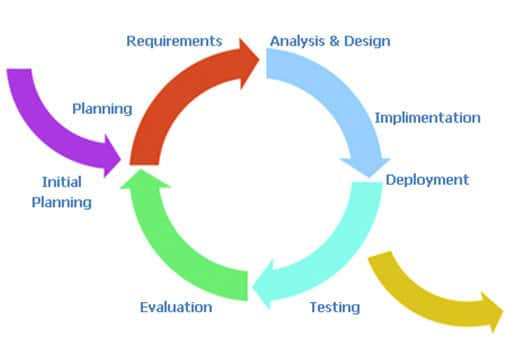
\includegraphics[]{images/cycle.png}
    		
    		\begin{center}
    			Figure 2.3: Incremental model for project
    		\end{center}
    	\end{figure}
    	After each cycle, backslide testing ought to be facilitated. Within the middle of this testing, harmed parts of the thing can be rapidly seen in light of the way that few changes are made interior any single emphasis. It is by and large simpler to test and explore than different strategies for programming movement in light of the way that for the foremost portion tinier changes are made within the middle of each emphasis. This mulls over more centred around and seriously testing of each portion interior the common thing. Client seem respond to highlights and overview the thing utilized for any required changes. Essential thing movement is faster and less costly in the incremental model.
    	
    	\section{Agility and Scrum}
    	Deft programming headway technique could be a strategy for making programming (like other programming alter systems - Waterfall appear, V-Model, Iterative show et cetera.) Be that as it may, dexterous framework moves in a common sense from different rationalities. In English, Dexterous implies 'ability to move rapidly and easily and reacting quickly to combination this is often a key piece of composed programming alters as well.
    	In traditionalist programming headway procedures like Waterfall illustrate, an errand can surrender different months and a long time to adequate as client might not get the chance to see last result till the perfection of the undertaking. At an unusual state, non-Agile assignments assign wide time frames for Prerequisites gathering, arrange, progression, testing and Client Acknowledgement Testing, sometime recently at final, sending the undertaking. In capability to this, Spry works out have Sprints or accentuations which are littler in term (Sprints/cycles can move from 2 weeks to 2 months) within the middle of which pre-chosen capabilities.
    	
    	\subsection{Agility and the cost of change}
    	The standard way of considering in programming progression (supported by numerous a long time of encounter) is that the fetched of advance increases nonlinearly as an undertaking progresses (Figure 2.3, solid dull twist). It is decently basic to oblige a alter when a item bunch is gathering prerequisites (right on time in a wander). A utilize circumstance must be changed, a rundown of capacities may well be broadened, or a composed specific can be changed. The costs of doing this work are immaterial, and the time required won't ominously impact the result of the undertaking. However, envision a situation where we fast forward different months. The bunch is amidst approval testing (something that happens for the most part late within the wander), and a basic accomplice is inquiring for a vital viable alter. The alter requires an change to the compositional arrange of the item, the diagram and advancement of three modern parts, alterations to another five segments, the system of unused tests, and so on.
    	
    	
    	\begin{figure}
    		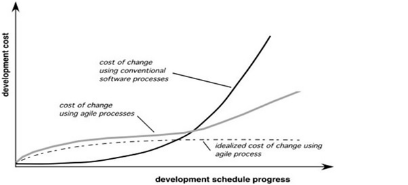
\includegraphics[]{images/chotu.png}
    		
    		\begin{center}
    				Figure 2.4: Agility and the cost of change
    		\end{center}
    	\end{figure}

    	\paragraph{}
    	\textbf{Advantages of Agile Methodology:}
    	\begin{itemize}
    		\item In Dexterous system the development of composing computer programs is unremitting.
    		\item The clients are fulfilled in light of the reality that after each Sprint working
    		component of the thing is passed on to them.
    		\item Clients can see of the working component which satisfied their needs.
    		\item In case the clients have any criticism or any change within the portion at that
    		point it can be obliged within the show section of the thing.
    		\item In Spry system the step by step affiliations are required between the masters
    		and the makers.
    		\item In this system thought is paid to the impressive graph of the thing.
    	\end{itemize}
    	
    	
    	
    	\section{Scrum}
    	Scrum could be a fast structure for coordinating work with a highlight on programming movement. It is arranged for get-togethers of three to nine fashioners who break their work into works out that can be done interior time boxed cycles, called runs (routinely two-weeks) and track advance and re-outline in 15-minute stand-up social undertakings, called step by step scrums. Ways to bargain with organizing made by diverse scrum bunches in more noteworthy afpucchi.pngfiliations solidify Large-Scale Scrum, Scaled Dexterous System (SAF) and Scrum of Scrums, among others.
    	
    	
    	\begin{figure}
    		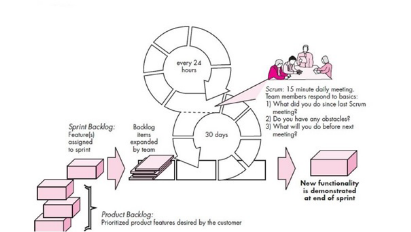
\includegraphics[]{images/animesh_chotu.png}
    		
    		\begin{center}
    			Figure 2.5: Scrum design of project
    		\end{center}
    	\end{figure}
		\paragraph{}
    	Scrum has three roles: Product Owner, Scrum Master, and Team:
    	\begin{itemize}
    		\item \textbf{Item Owner:} The Item Owner ought to beware of commerce with vision, ace, and openness. The Item Proprietor is responsible for persistently passing on the vision and necessities to the alter gathering. It's occasionally difficult for Product Proprietors to strike the proper alter of thought. Since Scrum respects self-relationship among social occasions, a Item Proprietor must battle the need. to littler scale direct. In the interim, Item Proprietors must be accessible to reply ask from the gathering.
    		
    		\item \textbf{Scrum Master:} The Scrum Master goes around as a aide for the Item Proprietor and the get-together. The Scrum Ace does not bargain with the social occasion. The Scrum Ace tries to cleanse any obstacles that are hindering the social issue from fulfilling its sprint destinations. This locks in the social occasion to remain imaginative and useful whereas guaranteeing its triumphs are clear to the Item Proprietor. The Scrum Ace other than tries to inquire the Item Proprietor around how to develop ROI for the social occasion.
    		
    		\item \textbf{Team:} As shown by Scrum's coordinator, "the gathering is completely self-managing." The progress total is capable for self-orchestrating to total work. A Scrum movement amass contains around seven completely devoted individuals (formally 3-9), in a perfect world in one gathering room ensured from exterior redirections. For programming meanders, a ordinary gathering solidifies a blend of programming engineers, modellers, programming engineers, examiners, QA experts, analysers, and UI organizers.
    	\end{itemize}
    	
    	
    	\section{Functional Requirements}
    	\begin{itemize}
    		\item Predict the probability of Heart Disease and Diabetes with given user inputs.
    		\item Contribute to the dataset or request to add functionalities.
    	\end{itemize}
    
    	
    	\section{Non-Functional Requirement}
    	\paragraph{}
    	Non-down to earth necessities are requirements that demonstrate criteria that can be used to judge the action of a structure, rather than specific practices. This could be showed up distinctively in connection to valuable requirements that describe specific direct or limits.
    	\paragraph{}
    	Non-down to earth necessities are a significant part of the time called attributes of a structure. Distinctive articulations for utilitarian necessities are confinements, quality characteristics, quality targets, nature of organization requirements and nonbehavioral essentials.
    	
    	\section{Feasibility Analysis}
    	\subsection{Technical feasibility} 
    	The project is technically feasible as it can be built using the existing available technologies. It is a web based applications that uses Grails Framework. The technology required by Disease Predictor is available and hence it is technically feasible.
    	
    	\subsection{Economic feasibility} 
    	The project is economically feasible as the cost of the project is involved only in the hosting of the project. As the data samples increases, which consume more time and processing power. In that case better processor might be needed.
    	
    	\chapter{Detailed Design}
    	This section will cover the design of our model in detail. Firstly with interface design that will provide a detailed explanation about the interface design, and then with the Data Structure and Algorithms that have been used in the project. The whole detailed system design with use case has been shown in Fig 3.1.
    	
    	\section{Interface Design}
    	This section describes about the user’s interaction with the interface. The inter-face designs/screen-shots have been added in order to give a better view of the user Interface.
    	
    	
    		\begin{center}
    			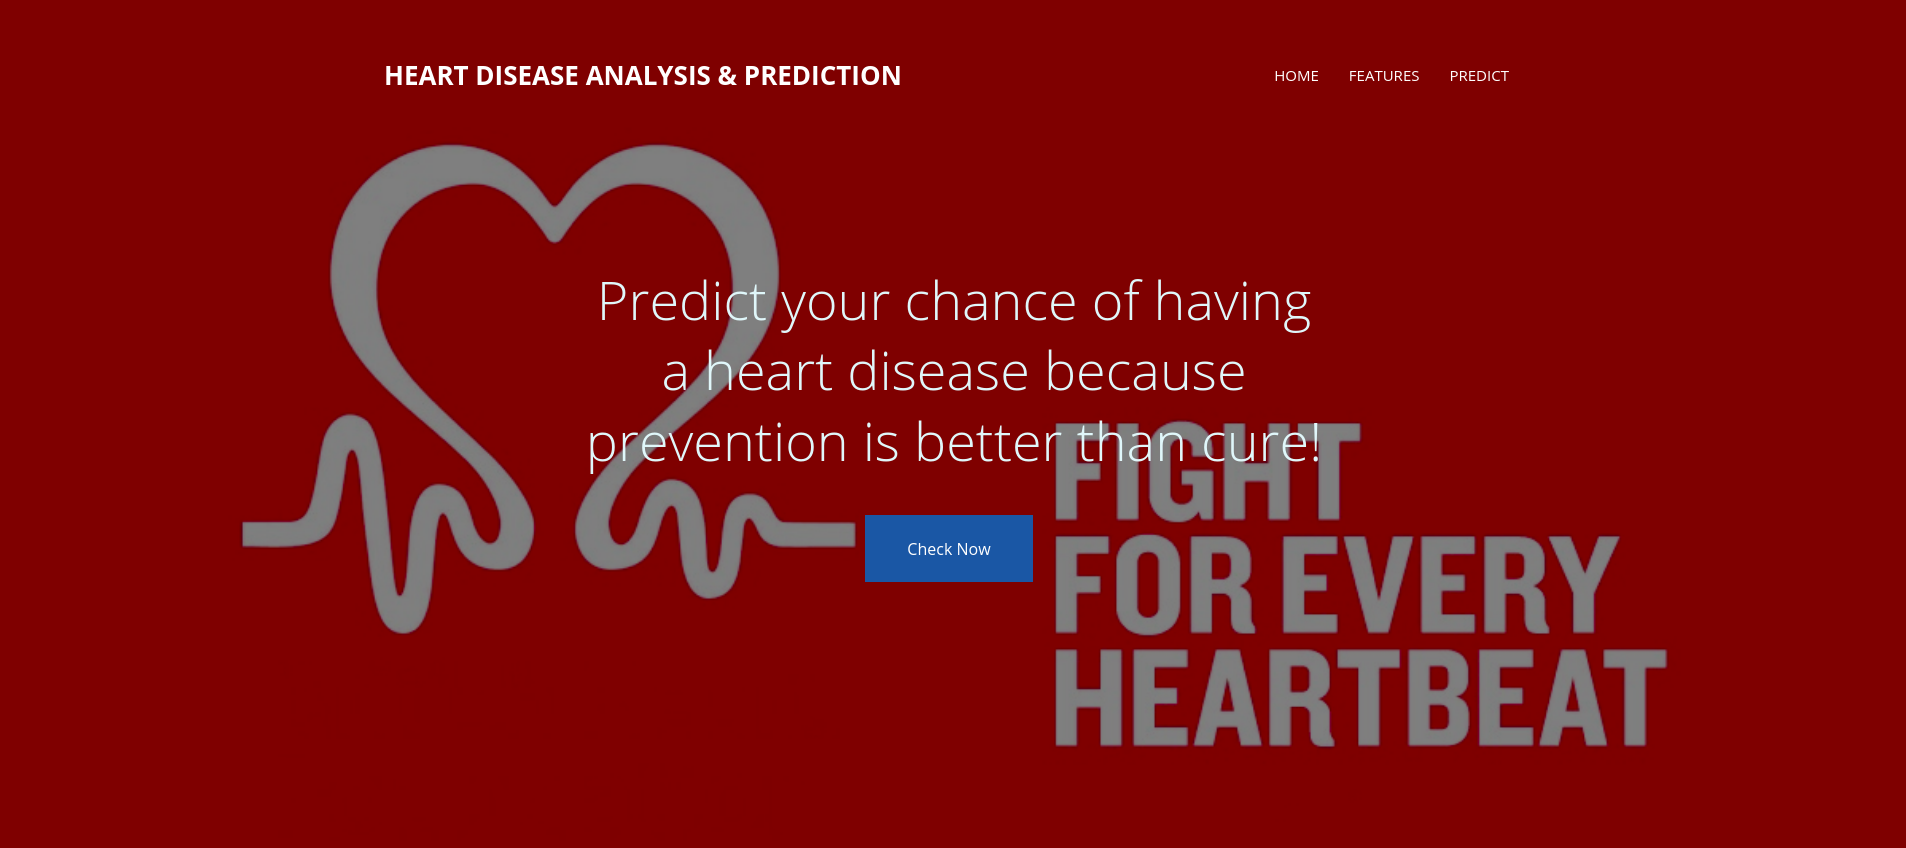
\includegraphics[width=17cm]{images/home.png}
    			\begin{figure}
    				\caption{Home page}
    			\end{figure}
    		\end{center}
    
    			
    			\begin{figure}
    				\begin{center}
    				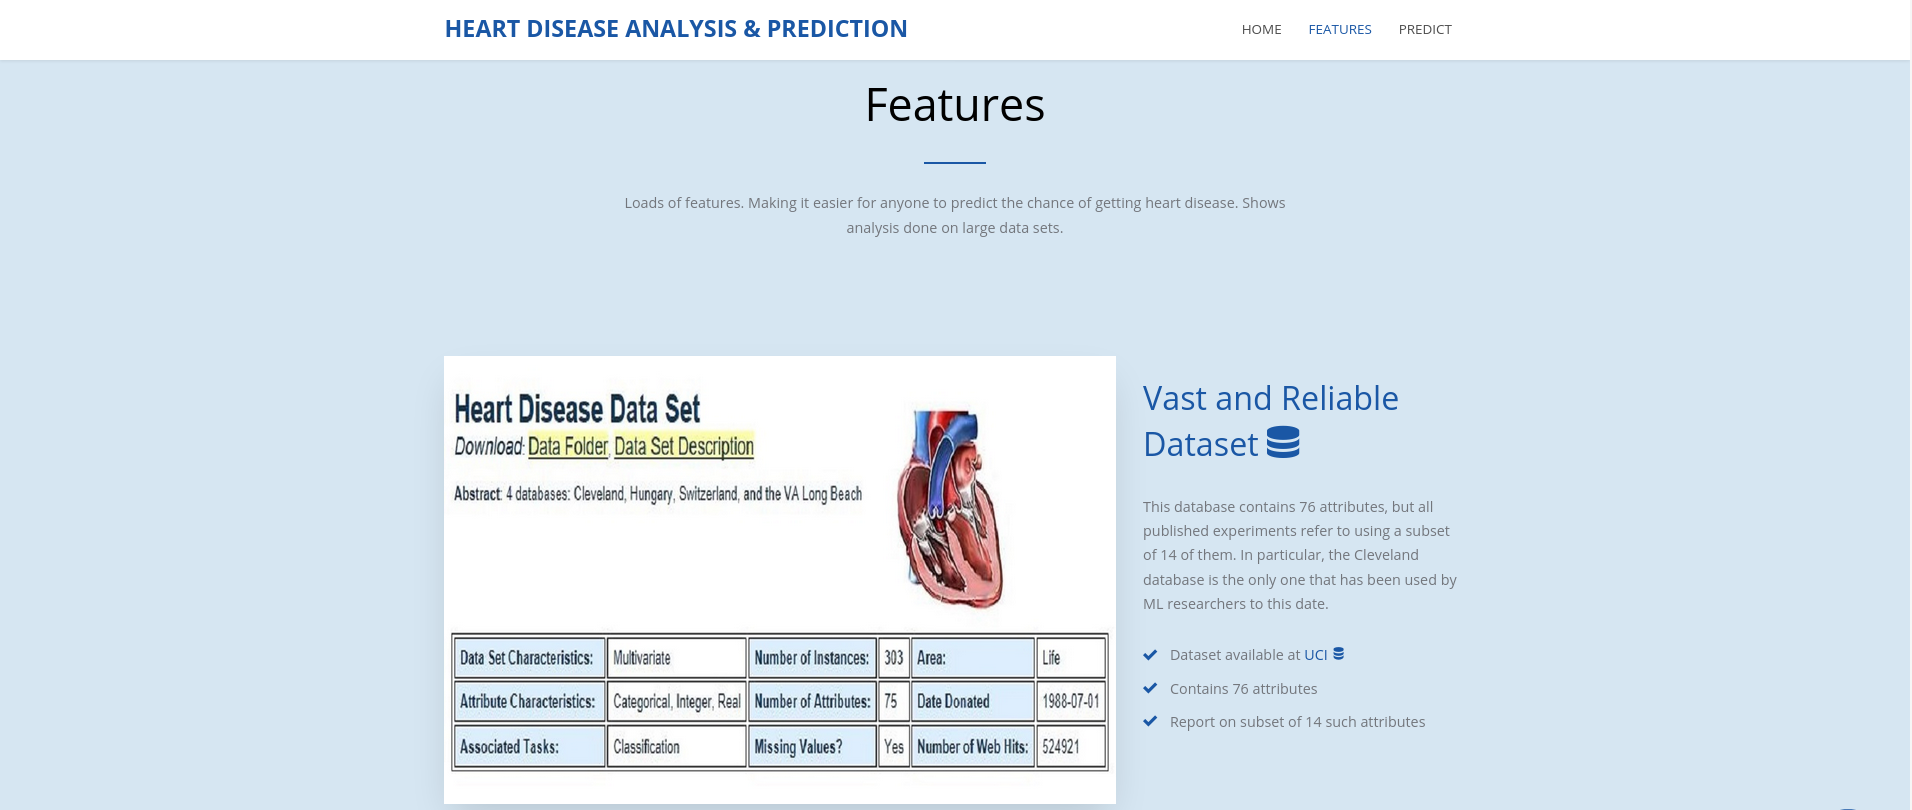
\includegraphics[width=17cm]{images/features}
    				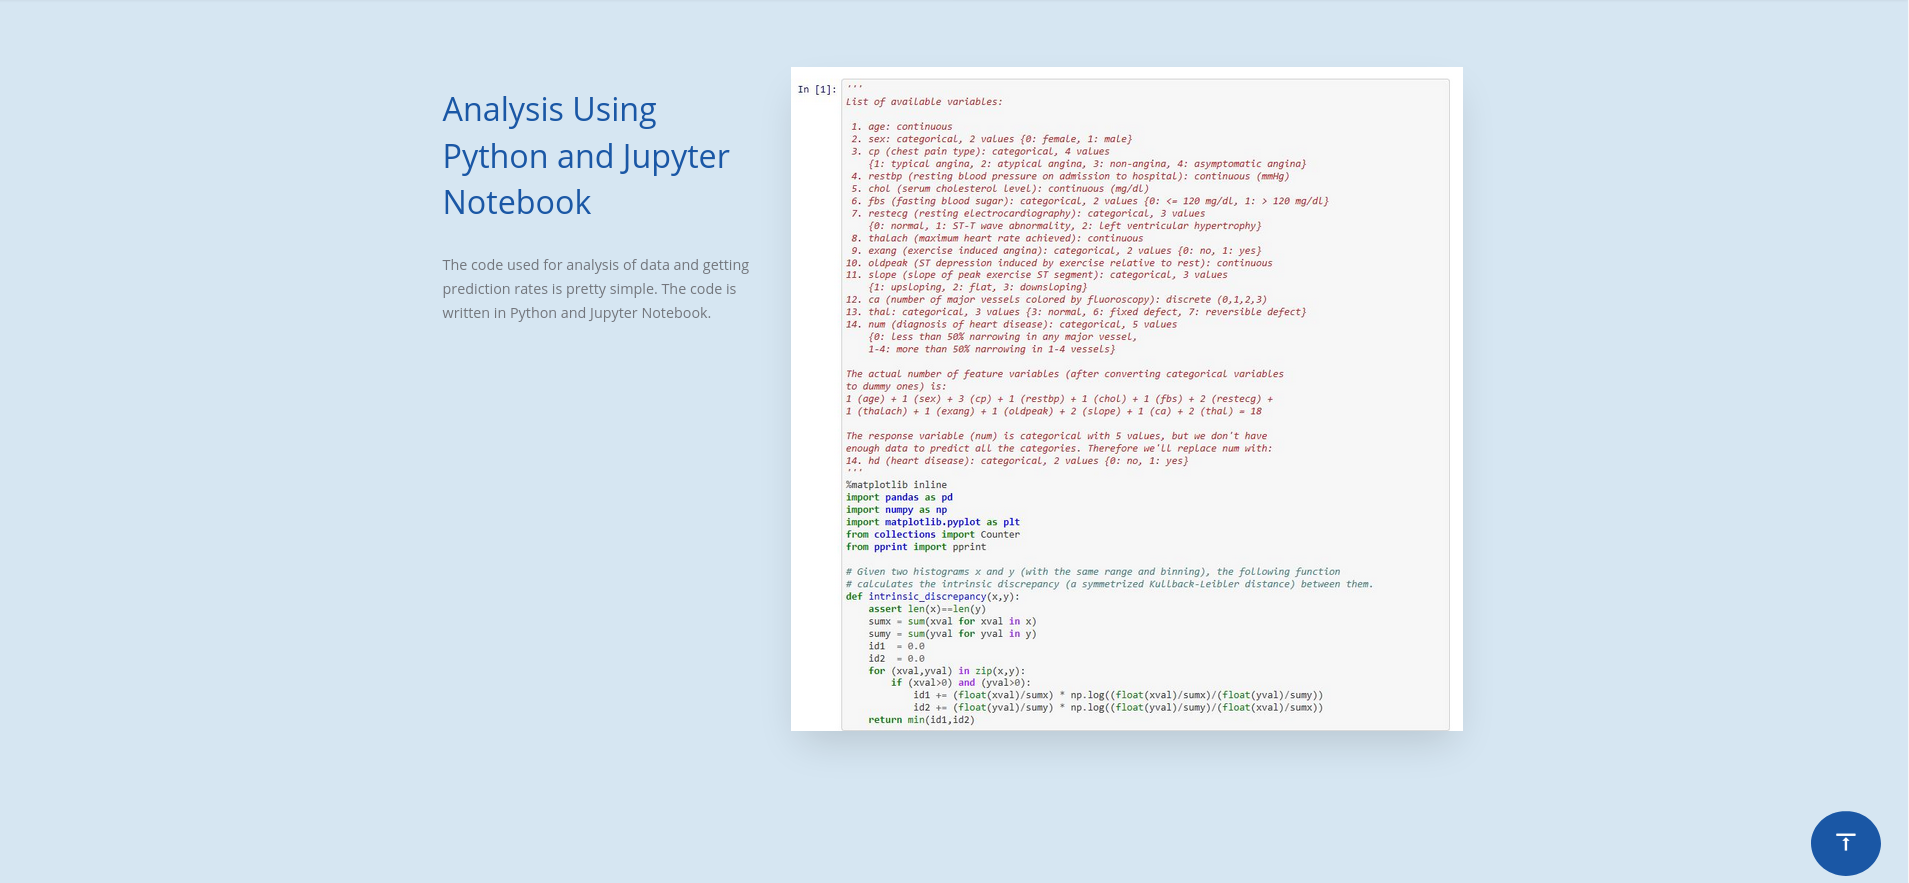
\includegraphics[width=17cm]{images/feature-analysis}
    				\caption{Feature of dataset}
    				\end{center}
    			\end{figure}
    			
    			\begin{figure}
    				\begin{center}
    				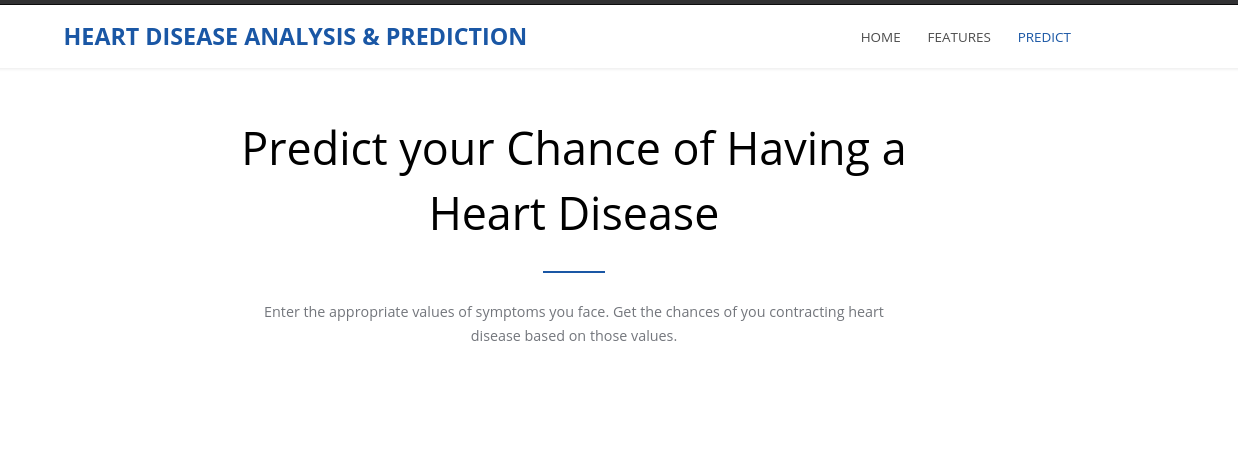
\includegraphics[width=17cm]{images/prediction-header}
    				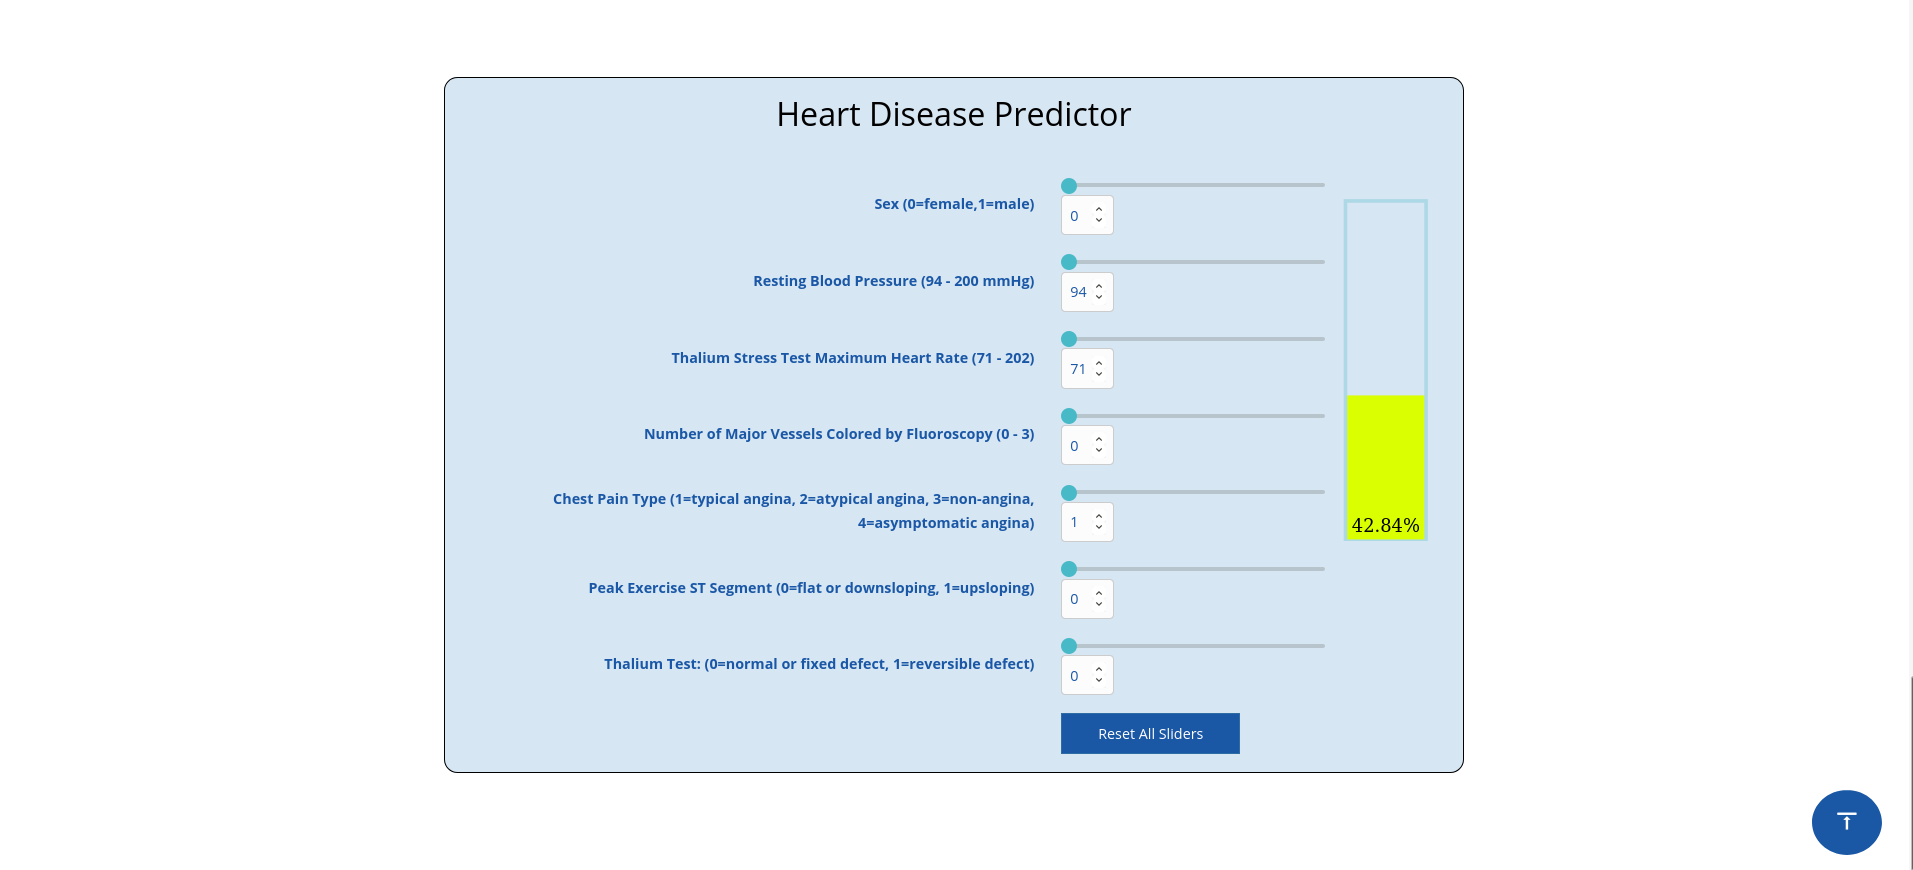
\includegraphics[width=17cm]{images/prediction}
    				\caption{Preiction Engine}
    				\end{center}
    			\end{figure}
    
    \pagebreak
    \section{Data Structures and Algorithms}
    	This section deals with data structure and algorithms we have used in our project.
    	
    \subsection{Naive Bayes Classifier}
    	Naive  Bayes  classifiers  are a  family  of  simple  probabilistic classifiers based by using Bayes theorem with strong (Naive) independence  assumptions between  the features.Naive  Bayes classifiers are highly  scalable by requiring a number  of  parameters  linear  for  the number  of  features  or predictors as variable in a learning problem. It is the simplest and the fastest probabilistic classifier especially for the training phase.\\
    	Naive Bayes classifier is based on Bayes theorem. This classifier uses conditional independence in which attribute value is independent of the values of other attributes. The Bayes theorem is as follows:
    	Let X= {x1, x2, ......, Xn} be a set of n attributes. In Bayesian, X is considered as evidence and H be some hypothesis means, the data of X belongs to specific class C. We have to determine P (H|X), the probability that the hypothesis H holds given evidence i.e. data sample X. According to Bayes theorem the P (H|X) is expressed as: \\
    	\[P(H|X) = \frac{P(X|H) * P(H)}{P(X)}\].
    	
    	\begin{figure}[h]
    		\begin{center}
    			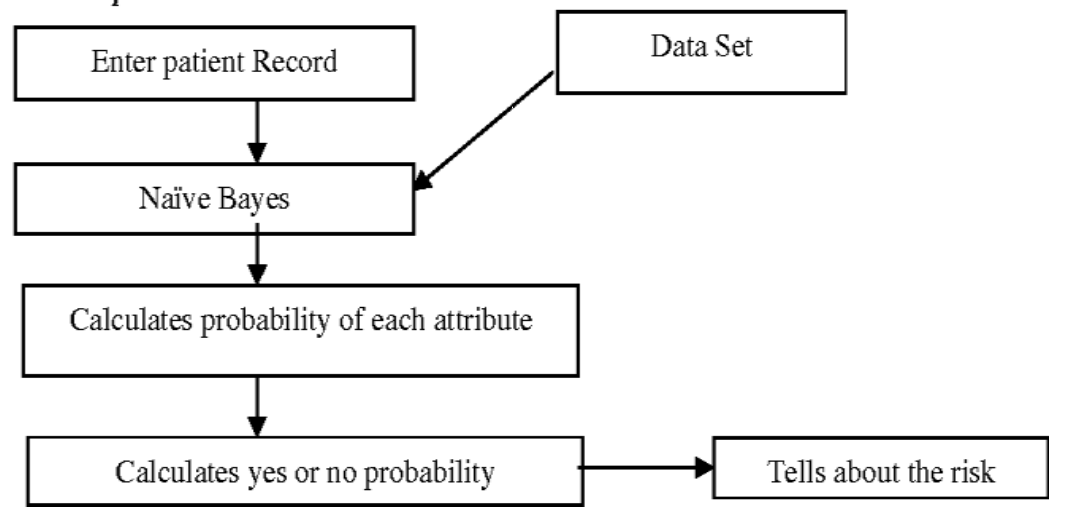
\includegraphics[width = 15cm]{images/naive_bayes.png}\\
    			\caption{Implementation Flow of Naive Bayes Algorithm}
    		\end{center}
    	\end{figure}
    	
       	Using Bayesian classifiers, the system will discover the concealed knowledge associated with diseases from historical records of the patients having heart disease. Bayesian classifiers predict the class membership probabilities, in a way that the probability of a given sample belongs to a particular class statistically. Bayesian classifier is based on Bayes’ theorem. We can use Bayes theorem to determine the probability that a proposed diagnosis is correct, given the observation. A simple probabilistic, the naive Bayes classifier is used for classification based on which is based on Bayes’ theorem. According to naive Bayesian classifier the occurrence or an occurence of a particular feature of a class is considered as independent in the presence or absence of any other feature. When the dimension of the inputs is high and more efficient result is expected, the chief Naive Bayes Classifier technique is applicable. The Naive Bayes model identifies the physical characteristics and features of patients suffering from heart disease. For each input, it gives the possibility of attribute of the acceptable state. Naive Bayes is a statistical classifier which assumes no dependency between attributes. This classifier algorithm uses conditional independence, means it assumes that an attribute value of a given class is independent of the values of other attributes. The advantage of using Naive Bayes is that one can work with the Naive Bayes model without. using any Bayesian methods. (Brownlee, 2016). 
    	P (Disease|symptom1, symptom2, ..., symptomn) P(Disease)P(symptom1, ..., symptomn|Disease) = P(symptom1, symptom2, ...symptomnN).\\
    	
    	
    
    
    	\subsection{Decision Tree}
    	Decision tree learning uses a decision tree as a predictive model which maps observations about an item to conclusions about the item's target value. It is one of the predictive modelling approaches used in statistics, data mining and machine learning. Tree models where the target variable can take a finite set of values are called classification trees. In these tree structures, leaves represent class labels and branches represent conjunctions of features that lead to those class labels. Decision trees where the target variable can take continuous values (typically real numbers) are called regression trees. In decision analysis, a decision tree can be used to visually and explicitly represent decisions and decision making. In data mining, a decision tree describes data but not decisions; rather the resulting classification tree can be an input for decision making.
    	The classification tree literally creates a tree with branches, nodes, and leaves that lets us take an unknown data point and move down the tree, applying the attributes of the data point to the tree until a leaf is reached and the unknown output of the data point can be determined. In order to create a good classification tree model, we need to have an existing data set with known output from which we can build our model. We also divide our data set into two parts: a training set, which is used to create the model, and a test set, which is used to verify that the model is accurate and not over fitted. \\
    	This classifier creates a decision tree based on which it assigns the class values to each data point. Here, we can vary the maximum number of features to be considered while creating the model.\\
    	
    		\begin{figure}
    		\begin{center}
    			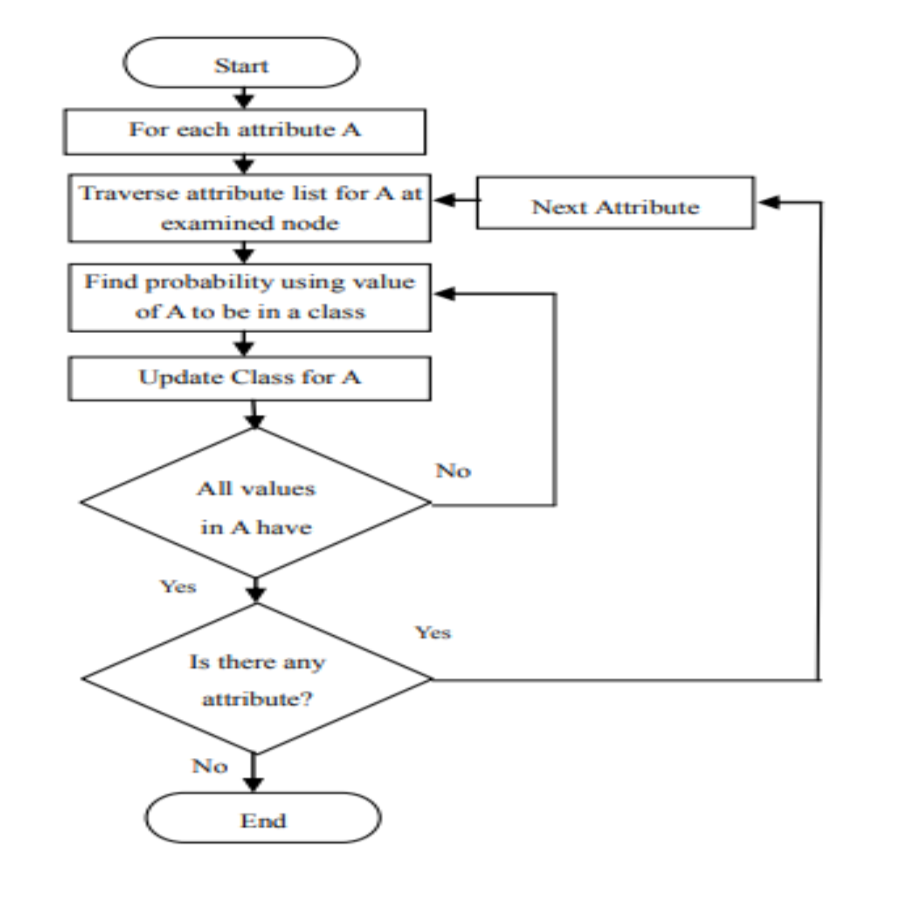
\includegraphics[height=17cm]{images/decision_tree.png}
    			\caption{Flowchart for Decision Tree}
    		\end{center}
    	\end{figure}
    
    	
    	\subsection{Support vector machine(SVM)}
    	SVM was developed by Vladimir Vapnik at AT\&T Bell Labs. It is based on the concept of decision planes that define decision boundaries. A decision plane is a hyperplane that separates the objects having different class memberships. SVM classifiers separate the observations into two or more classes in such a way that maximum separation is achieved. A hypothetical hyperplane is the separator in SVM classification problems.  In other words, SVM constructs a hyperplane that separates the two sets so as to minimize the number of misclassified points. Generally, there are two types of SVM models: linear and nonlinear. Linear SVM works better on linearly separable datasets but nonlinear SVM model works well even on hardly separable datasets. Since we are dealing with hardly separable data in our experiments we use nonlinear SVM. The dual formulation of the nonlinear SVM function can be formulated as
    	\[ MaxW(\alpha) = \sum_{i=1}^{m}\alpha_i - 0.5\sum_{i, j=1}^{m}\alpha_i \alpha_j y_i y_j K(x_i . x_j) \]\\
    	subject to:
    	\[\sum_{i=1}^{m}\alpha_i y_i = 0 ,\]\\
    	\[ 0 \leq \alpha_i \leq C \]\\
    	\begin{figure}
    		\begin{center}
    			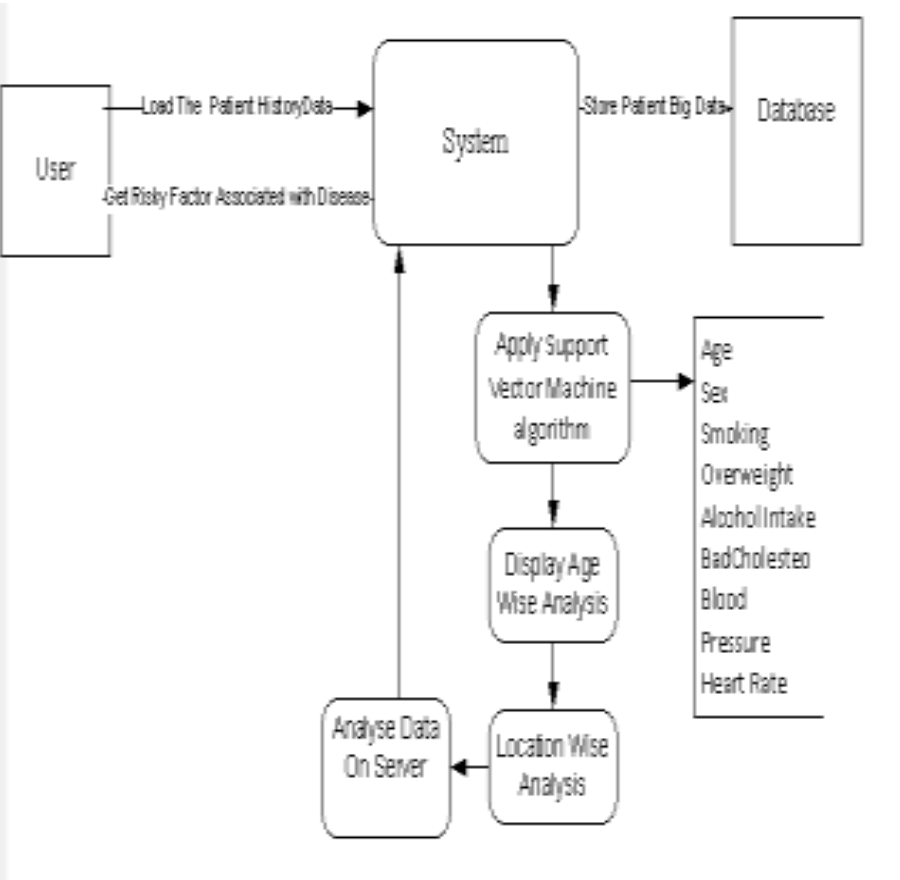
\includegraphics[width=14cm]{images/svm.png}
    			\caption{Flowchart For SVM}
    		\end{center}
    	\end{figure}
    	Input vectors $x_i \in R^m$ , i= 1, 2, 3, …, m, which are called features or attributes are extracted from the database. Associated with every particular input we have a corresponding label ($ y_i = \pm 1$) which is called the target value or output in the database. The variable $\alpha_i$ is the Lagrange multiplier in the dual formulation and C is a user-specified parameter representing the penalty for misclassification K(xi ,xj) is the kernel function and maps the original data points to another space.  One of the popular choices for the kernel is Gaussian kernel which is also known as Radial Basis Function (RBF) in the literature. The formulation for this kernel is
    	\[ K(x_i, x_j) = e^{-\frac{\parallel{x_i - x_j}\parallel^2}{2\sigma}} \]
    	where parameter $\sigma$ is known as the kernel width. 
    	
    	
    	
    	\subsection{Logistic Regression}
    	Logistic Regression is a statistical analysis technique that is used for predicting the data value based on the prior observation of the data set. The logistic regression model predicts the dependent data variable by analyzing the relationship between one or more existing independent variables. Logistic Regression is one of the important tools for prediction, which can also be used for classifying and predicting the data based on the historical data. The implemented model is a binary Logistic model that has dependent variables with only two possible outcomes i.e., one is a positive value and another one is the negative value which is having 0 or 1 as a class label.
    	It mainly consists of two major phases: regularized cost function and regularized gradient descent. Cost Function is used for calculating the maximum likelihood estimation. Gradient descent is an iterative process for getting coefficients from training
    	data. The process is repeated until we get the optimal parameters of train data. The model is trained with the optimal coefficient.Whenever a test data has been passed to the model based on the parameters is able to identify whether the person is having heart disease or not, it tests the data using the sigmoid function. The cost function is the method that is used for reducing the errors of the predicted label and the actual label. Gradient descent function is the method that is used for calculating the coefficient until we obtain a minimum value of the class label.
    	
    		
    	\begin{figure}
    		\begin{center}
    			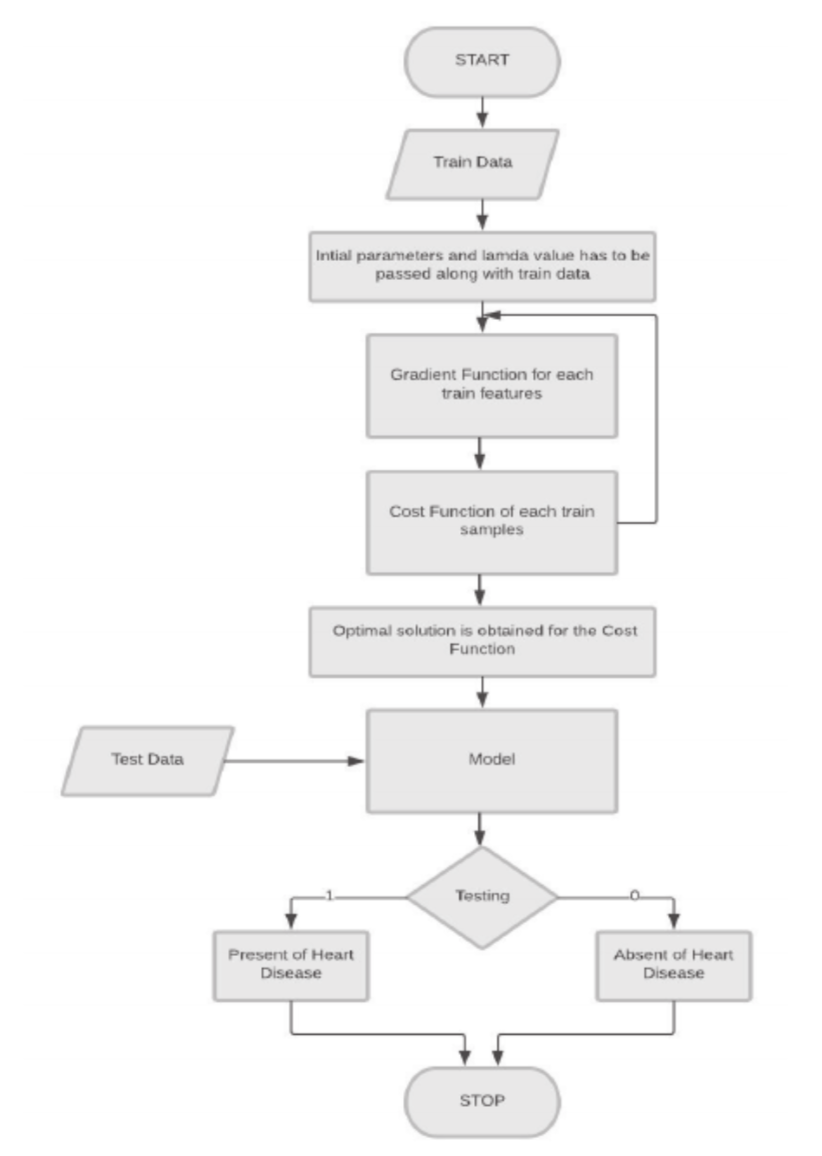
\includegraphics[width=14cm]{images/logistic_regression.png}
    			\caption{FlowChart For Logistic Regression}
    		\end{center}
    	\end{figure}
    	
    	\subsubsection{Cost Function}
    		A minimization function is used that is the cost function. It uses the 
    		Log Loss i.e. the logarithmic loss which measures the performance 
    		of the model where the prediction input value is the probability 
    		between the zero and one. The Log loss is the uncertainty of the 
    		prediction which is based on the how  much  it  varies  from  the 
    		actual label. Cost function which helps the learner to correct or 
    		change the behavior to minimize the mistakes. The cost function 
    		can be estimated by iteratively running the model to compare the 
    		estimated predicted value and the known or actual  value. The 
    		regularized cost function is a method that is used for overcoming 
    		the risk of over fitting.  Lamda  is  the  parameter  which  controls 
    		the regularization term. The  cost function  is calculated  by  the 
    		following:
    		\[ J(\theta) = \frac{1}{m}\sum_{i=1}^{m} y^{(i)} \log[h_\theta(x^{(i)}) - (1-y^{(i)}) \log(1-h_\theta(x^{(i)})] + \frac{\lambda}{2m}\sum_{i=1}^{n}{\theta_j}^2 \] \\
    		m = number of instances \\
    		n = number of attributes \\
    		y = class label \\
    		x = train data features\\
    		$\theta$ = coefficients \\ 
    		$\lambda$ =learning rate
    	
    	
    	\subsubsection{Gradient Descent}
    		Gradient descent is an optimization method which is used to find 
    		the parameters or  the  coefficient  of  the  cost  function.  Gradient 
    		descent is  a  repeated  process  in  order  to  get  the  coefficients  to 
    		minimize the cost function. The  Gradient  descent  is  calculated 
    		for both the classes to get the pair of a coefficient for both class 
    		labels. The goal here is to continue the procedure to try the different 
    		value for the coefficient, evaluating their cost  and selecting the new coefficient that is having the slightly lower cost. Considering this coefficient and storing them in the model. Gradient descent 
    		is calculates as the following:
    		\[ \theta_{ji} = \theta_j - \frac{1}{m}\sum_{i=1}^{m}(h_\theta(x^i)-(y^i)) {x_j}^i + \frac{\lambda}{m} \theta_j \]\\
    		m = number of instances \\
    		x = train data features \\
    		y = class label \\
    		$\theta$ = coefficients \\
    		$\lambda$ = learning rate 
    		
    		
    
    	\subsubsection{Sigmoid Function}
    		Sigmoid function is the logistic function between. This takes the 
    		real input vales and output values between the 0 and 1 for logistic 
    		function [12]. This is interpreted as taking log odds and having 
    		the output probability. Generally sigmoid function is used to map 
    		predictions to probability it is defined as:
    		\[ h_\theta(x) = \frac{1}{1 + e^{-\theta^{T.x}}} \]\\
    		x = test data features \\
    		$\theta$ = coefficients 
    		Whenever a  test  data is passed it calculates  the  value based on 
    		the parameters stored in the model. It calculates the probability 
    		of each class label. We return the maximum probability value of 
    		the class label $x_i$.\\
    		The test data contains the thirteen attributes that we need to pass 
    		and calculate   for both  the classes it will return  the two values 
    		we take the maximum value of two values we will return the class 
    		label which is having the maximum probability.
    	
    	
    	
    		
    		\subsection{K-Nearest Neighbour}  
    		K-Nearest neighbor (KNN) is a simple, lazy and nonparametric classifier. KNN is preferred when all the features are continuous. KNN is also called case-based reasoning and has been used in many applications like pattern recognition, statistical estimation. Classification is obtained by identifying the nearest neighbor to determine the class of an unknown sample. KNN is preferred over other classification algorithms due to its high convergence speed and simplicity.\\
    		KNN classification has two stages
    		\begin{enumerate}
    			\item Find the k number of instances in the dataset that is closest to instance S
    			\item These k number of instances then vote to determine the class of instance S
    		\end{enumerate}
    		The Accuracy of KNN depends on distance metric and K value. Various ways of measuring the distance between two instances are cosine, Euclidean distance. To evaluate the new unknown sample, KNN computes its K nearest neighbors and assign a class by majority voting.\\    		
    		With KNN algorithm, we have chance to change the parameter's weight. It means that, we may assume that some parameters are more important or making more impact than others. Among 8 parameters we use, we can categorize them our data into 2 categories, one is "non-medical" parameters (Age and Sex) and the other is "medical" parameters (CP, Trestbps, Trestbpd etc). We may think that medical parameters are more important than non medical, which we will see in experimental results. Along with weighting, we should find the value of "k" so it gives the best classification result. Since it is a 2-choice classification ("yes") and (“No”) k will be an odd number.
    		
    		\begin{figure}
    			\begin{center}
    				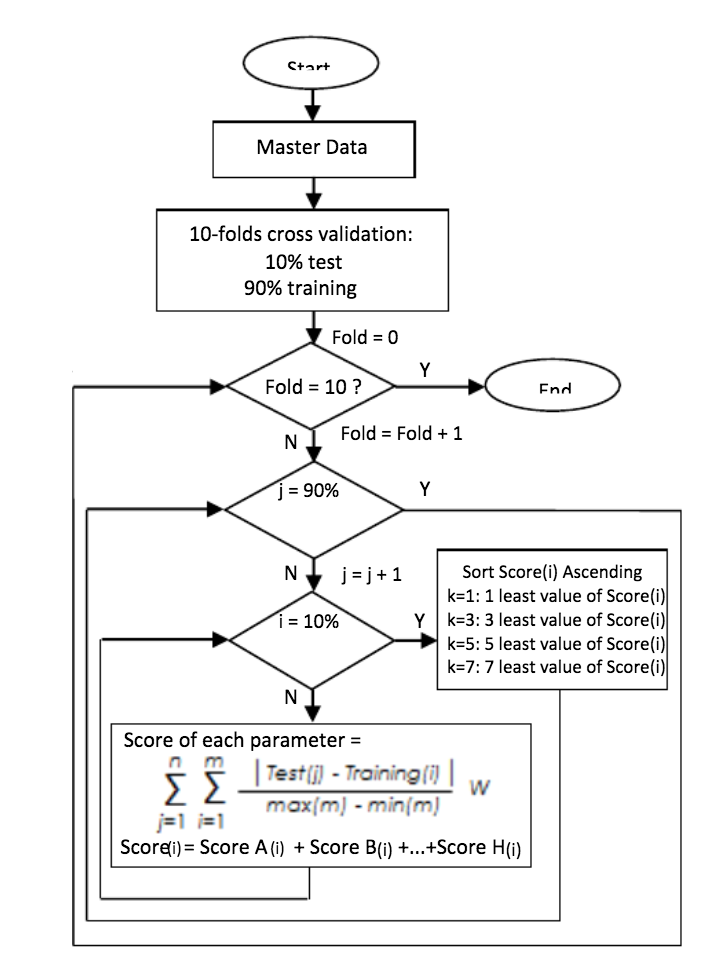
\includegraphics[width=15cm]{images/knn.png}
    				\caption{FlowChart for KNN}
    			\end{center}
    		\end{figure}
    
  		\subsection{Neural Network}
  		\subsubsection{Multilayer Perceptron Neural Network (MLPNN)}
  		One of the most important models in Artificial Neural Network is Multilayer Perceptron
  		(MLP). The  type of architecture  used to  implement  the system  is Multilayer Perceptron Neural Network (MLPNN).
  		\begin{figure}[H]
  			\begin{center}
  				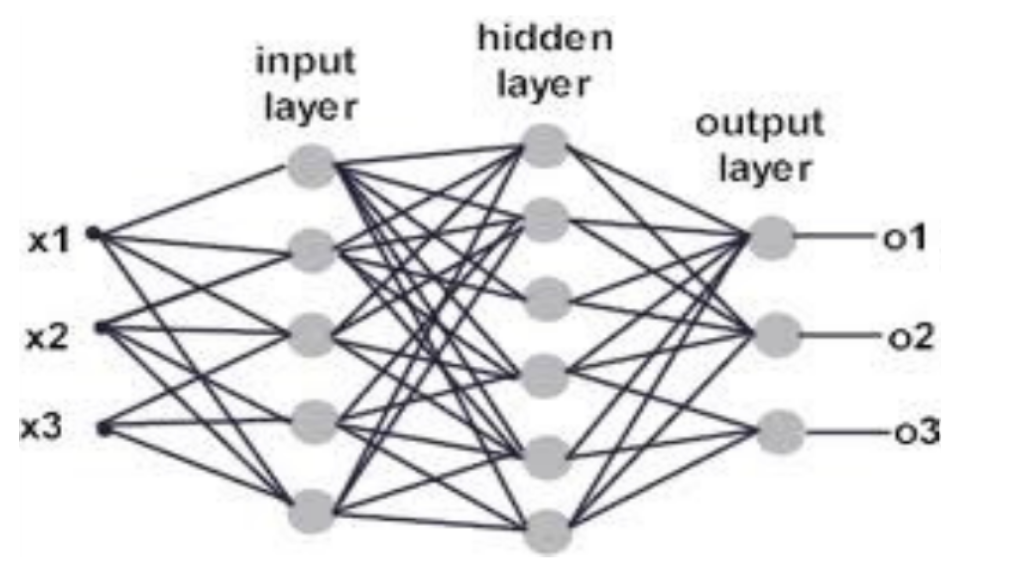
\includegraphics[width=12cm]{images/mlpnn.png}
  			\end{center}
  		\end{figure}
  		The MLPNN consists of one input layer, one output layer and one or more hidden layers.Each layer consists of one or more nodes, represented by small circles. The lines between nodes indicate flow of information from one node to another node. The input layer receives signals from external nodes. The output of input layer is given to hidden layer, through weighted connection links. It performs computations and transmits the result to output layer through weighted links. The output of hidden layer is forwarded to output layer, it performs computations and produce final result. The working of multilayer perceptron neural network is summarized in steps as mentioned
  		Below:
  		\begin{enumerate}
  			\item Input data  is provided to input layer for processing, which  produces a
  			predicted output.
  			\item The predicted output is subtracted from actual output and error value is
  			calculated.
  			\item  The network then  uses a  Backpropagation algorithm  which  adjusts the
  			weights.
  			\item For weights adjusting it starts from weights between output layer nodes
  			and last hidden layer nodes and works backwards through network.
  			\item When back propagation is finished, the forwarding process starts again.
  			\item The process is repeated until the error between predicted and actual output
  			is minimized.
  		\end{enumerate}
  	
  	\subsubsection{Backpropagation network}
  	The most widely used training algorithm for multilayer and feed forward network is
  	Backpropagation. The name given is back propagation because it calculates the difference between actual and predicted values is propagated from output nodes backwards to nodes in previous layer. This is done to improve weights during processing.The working of Backpropagation algorithm is summarized in steps as follows:
  	\begin{enumerate}
  		\item Provide training data to the network.
  		\item Compare the actual and desired output.
  		\item Calculate the error in each neuron. 
  		\item Calculate what output should be for each neuron and how much lower or
  		higher output must be adjusted for desired output.
  		\item Then adjust the weights
  	\end{enumerate}
  
  \begin{figure}
  	\begin{center}
  			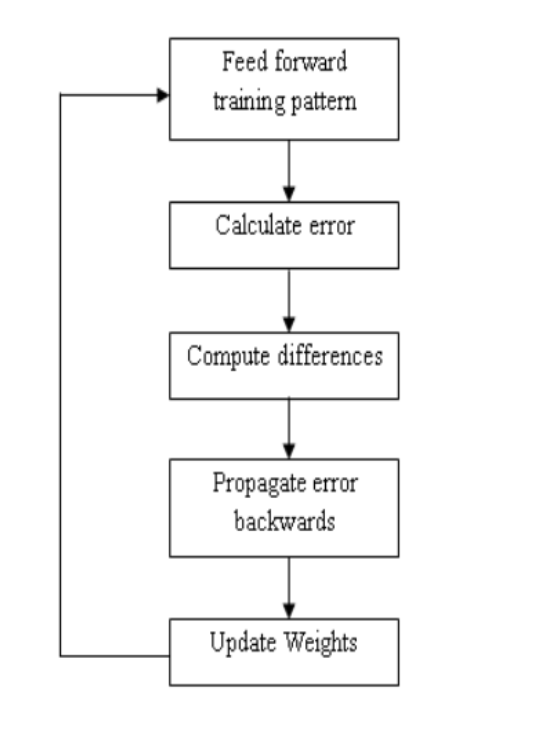
\includegraphics[width=8cm]{images/backpropogation.png}
  	\end{center}
  \end{figure}

\begin{figure}
	\begin{center}
		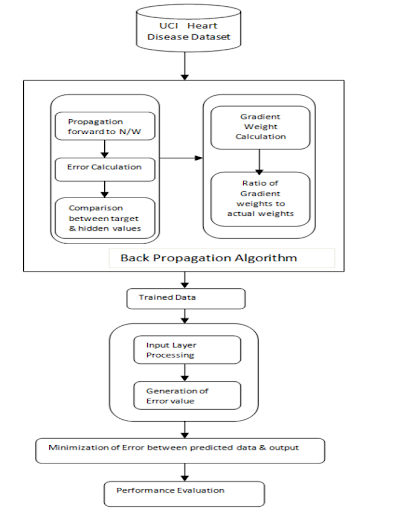
\includegraphics[width=10cm, height=20cm]{images/neural_network.png}
		\caption{Flowchart for Neural Network}	
	\end{center}
\end{figure}

	\section{UML diagrams with discussions}
  	
  	\section{Data Source/Database used and Formats}
  	\subsection{Heart Disease DataSet}
  	The dataset used in this project is the Cleveland Heart Disease dataset taken 
  	from the UCI repository.
  	\begin{center}
  		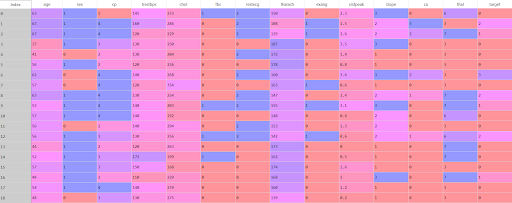
\includegraphics[width=15cm]{images/hdDataset.png}
  	\end{center}
  
  The dataset consists of 303 individuals data. There are 14 columns in the dataset, which    are described below.
  \begin{enumerate}
  	\item\textbf{Age:} displays the age of the individual.
  	
  	\item \textbf{Sex:} displays the gender of the individual using the following format :
  		\begin{itemize}
  			\item 1 = male
  			\item 0 = female
  		\end{itemize}
  	
  	\item \textbf{Chest-pain type:} displays the type of chest-pain experienced by the individual using the following format :
  		\begin{itemize}
  			\item 1 = typical angina
  			\item 2 = atypical angina
  			\item 3 = non — anginal pain
  			\item 4 = asymptotic
  		\end{itemize}
  
  	\item \textbf{Resting Blood Pressure}: displays the resting blood pressure value of an individual in mmHg (unit)
  	
  	\item \textbf{Serum} Cholestrol: displays the serum cholesterol in mg/dl (unit)
  	
  	\item \textbf{Fasting Blood Sugar}: compares the fasting blood sugar value of an individual with 120mg/dl.
  		\begin{itemize}
  			\item If fasting blood sugar > 120mg/dl then : 1 (true)
  			\item else\\ 								   : 0 (false)
  		\end{itemize}
  	
  	\item \textbf{Resting ECG:} displays resting electrocardiographic results
  	\begin{itemize}
  		\item 0 = normal
  		\item 1 = having ST-T wave abnormality
  		\item 2 = left ventricular hyperthrophy
  	\end{itemize}
  	
  	\item \textbf{Max heart rate achieved:} displays the max heart rate achieved by an individual.
  	\item \textbf{Exercise induced angina} :
	  	\begin{itemize}
  			\item 1 = yes
  			\item 0 = no
  		\end{itemize}
  	
  	\item \textbf{ST depression induced by exercise relative to rest:} displays the value which is an integer or float.
  	
  	\item \textbf{Peak exercise ST segment:}
  		\begin{itemize}
	  		\item 1 = upsloping
  			\item 2 = flat
  			\item 3 = downsloping
 	 	\end{itemize}
  	
  	\item \textbf{Number of major vessels (0–3) colored by flourosopy :} displays the value as integer or float.
  	
  	\item \textbf{Thal :} displays the thalassemia :
  		\begin{itemize}
  			\item 3 = normal
  			\item 6 = fixed defect
  			\item 7 = reversible defect
  		\end{itemize}
  	
  	\item \textbf{Diagnosis of heart disease :} Displays whether the individual is suffering from heart disease or not :
  	\begin{itemize}
  		\item 0 = absent
  		\item 1, 2, 3, 4 = present.
  	\end{itemize}
  	
  \end{enumerate}
  	
  
  	
  		

\end{document}


